\begin{question}
\noindent A games map designer is testing symmetry rules for a Valorant-style tactical map editor. A rectangular control zone $PQRS$ is drawn on the design grid, together with the line $y = x$ and the origin $O$.

\begin{center}
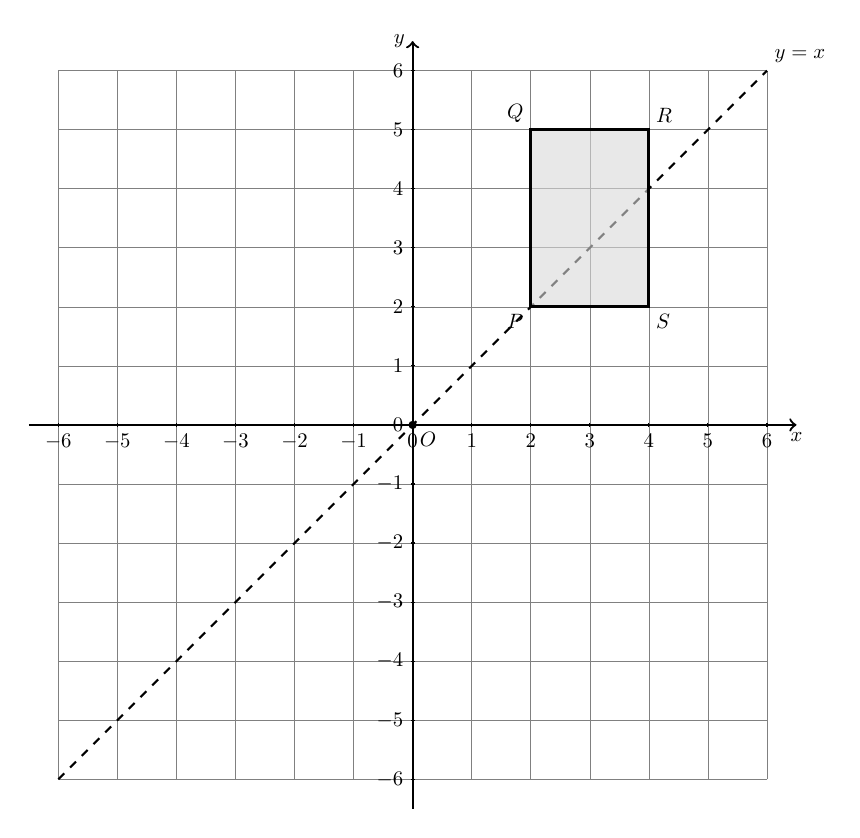
\begin{tikzpicture}[scale=0.75, transform shape]
    \def\axisLimit{6}

    \definecolor{borderColour}{HTML}{000000}
    \definecolor{fillColourA}{HTML}{D8D8D8}

    % Draw grid
    \draw[step=1cm,gray,very thin] (-\axisLimit,-\axisLimit) grid (\axisLimit,\axisLimit);

    % Draw axes
    \draw[thick,->] (-\axisLimit-0.5,0) -- (\axisLimit+0.5,0) node[anchor=north] {$x$};
    \draw[thick,->] (0,-\axisLimit-0.5) -- (0,\axisLimit+0.5) node[anchor=east] {$y$};

    % Label x-axis and y-axis
    \foreach \x in {-\axisLimit,...,\axisLimit}
        \draw (\x cm,1pt) -- (\x cm,-1pt) node[anchor=north] {$\x$};
    \foreach \y in {-\axisLimit,...,\axisLimit}
        \draw (1pt,\y cm) -- (-1pt,\y cm) node[anchor=east] {$\y$};

    % Draw the line y = x
    \draw[thick,dashed] (-6,-6) -- (6,6) node[anchor=south west] {$y=x$};

    % Rectangle PQRS: P(2,2), Q(2,5), R(4,5), S(4,2)
    \coordinate (P) at (2,2);
    \coordinate (Q) at (2,5);
    \coordinate (R) at (4,5);
    \coordinate (S) at (4,2);

    \filldraw[fill=fillColourA, draw=borderColour, line width=1pt, fill opacity=0.6] (P) -- (Q) -- (R) -- (S) -- cycle;

    \node[below left] at (P) {$P$};
    \node[above left] at (Q) {$Q$};
    \node[above right] at (R) {$R$};
    \node[below right] at (S) {$S$};

    \fill[black] (0,0) circle (2pt);
    \node[below right] at (0,0) {$O$};

\end{tikzpicture}
\end{center}

\noindent The rectangle $PQRS$ has vertices $P(2,2)$, $Q(2,5)$, $R(4,5)$ and $S(4,2)$.

\noindent The rectangle is first reflected in the line $y = x$ to give rectangle $P_1Q_1R_1S_1$.

\noindent Rectangle $P_1Q_1R_1S_1$ is then rotated $180^\circ$ about the origin $O$ to give rectangle $P_2Q_2R_2S_2$.

\noindent By considering the effect of \textbf{both} transformations on each vertex of $PQRS$, find the coordinates of any point(s) on the perimeter of the rectangle that are invariant under the \textbf{combined} transformation (reflection in $y=x$ followed by rotation $180^\circ$ about $O$).

\vspace{5cm}

\begin{flushright}
    \answerlines{5}{3}
\end{flushright}
\end{question}